
\documentclass{article}

\usepackage{fullpage}
\usepackage{graphicx}
\usepackage{amsmath}
\usepackage{textcomp}

\title{Wave Equation Simulation}
\author{Michael Deakin}

\begin{document}
\maketitle

\begin{section}{Introduction}
In this report, I describe the properties of the solvers written for the wave equation.
The primary solver used in this report used $2^{nd}$ order upwinding spatial discretization
and RK2 for the time discretization, though I also implemented $1^{st}$, $3^{rd}$,
and $4^{th}$ order timestepping, in addition to a $1^{st}$ order spatial discretization.
\end{section}

\begin{section}{Verification}
Verification of correctness of the solver was primarily ensured through the use of unit tests.
These ensured that the maximum error of the flux, the flux integral,
and the timesteps were all less than a threshold and eventually converged to the expected answer
(with the expected order) for some cases with known solutions.
This ensures that the logic in the code is internally consistent.
To ensure external consistency, I plotted the solvers output to verify it looked as expected,
and also plotted the error against a known solution.
The plots of the errors when run with 20, 40, and 80 control volumes with RK1 and RK2
are shown in Figure \ref{rk_errors}.
As expected, the error is low near the left boundary and increases to the right.
Also as expected, the error appears to go to zero at $1^{st}$ (ie, linearly)
and $2^{nd}$ (quadratically) order rates for the RK1 and RK2 solvers, respectively.
\begin{figure}[ht]
  \centering{
    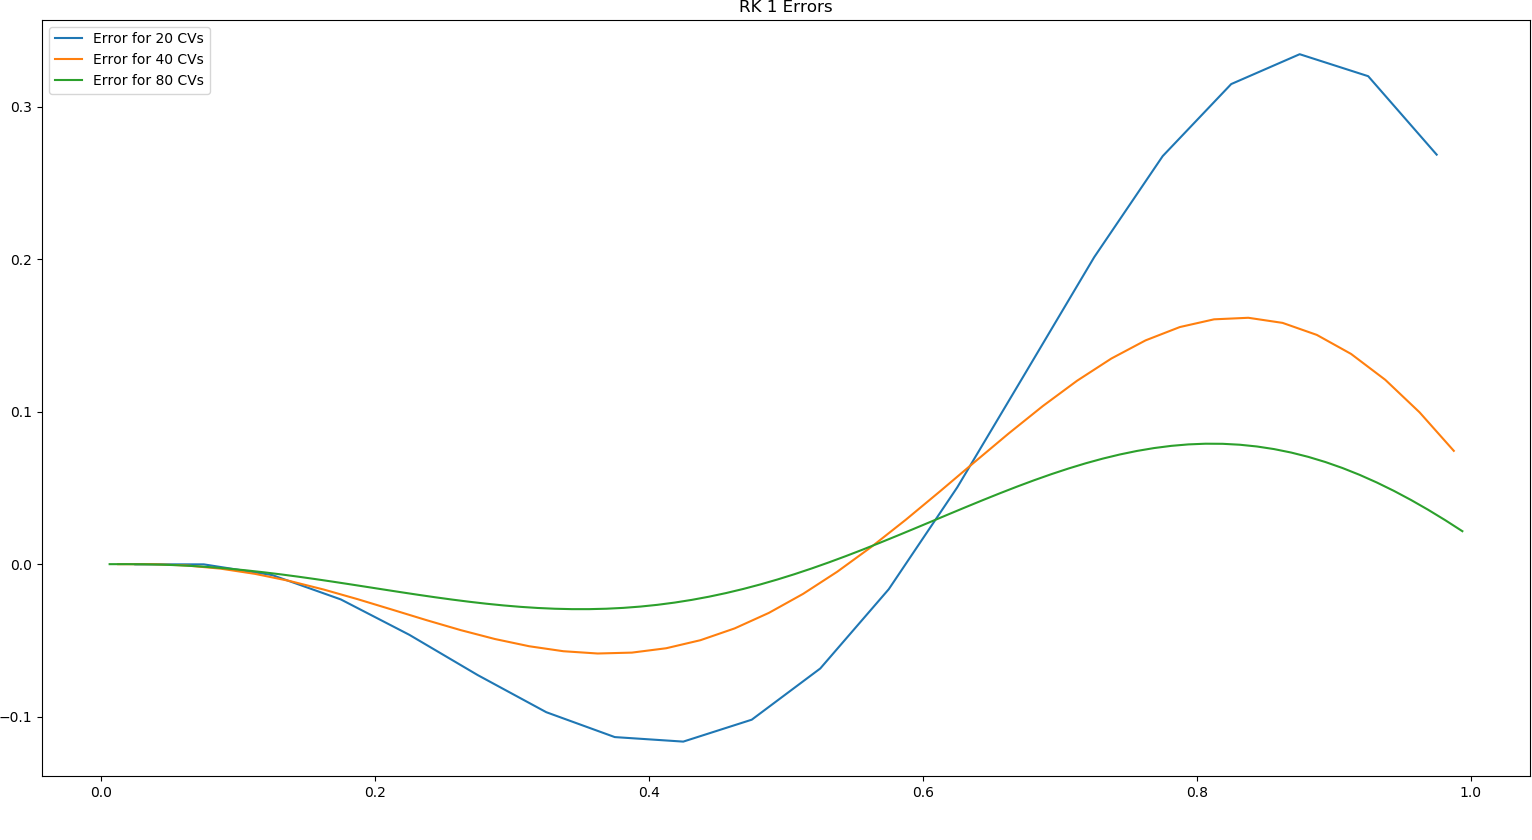
\includegraphics[width=0.7\textwidth]{figs/part1_rk1.png}
    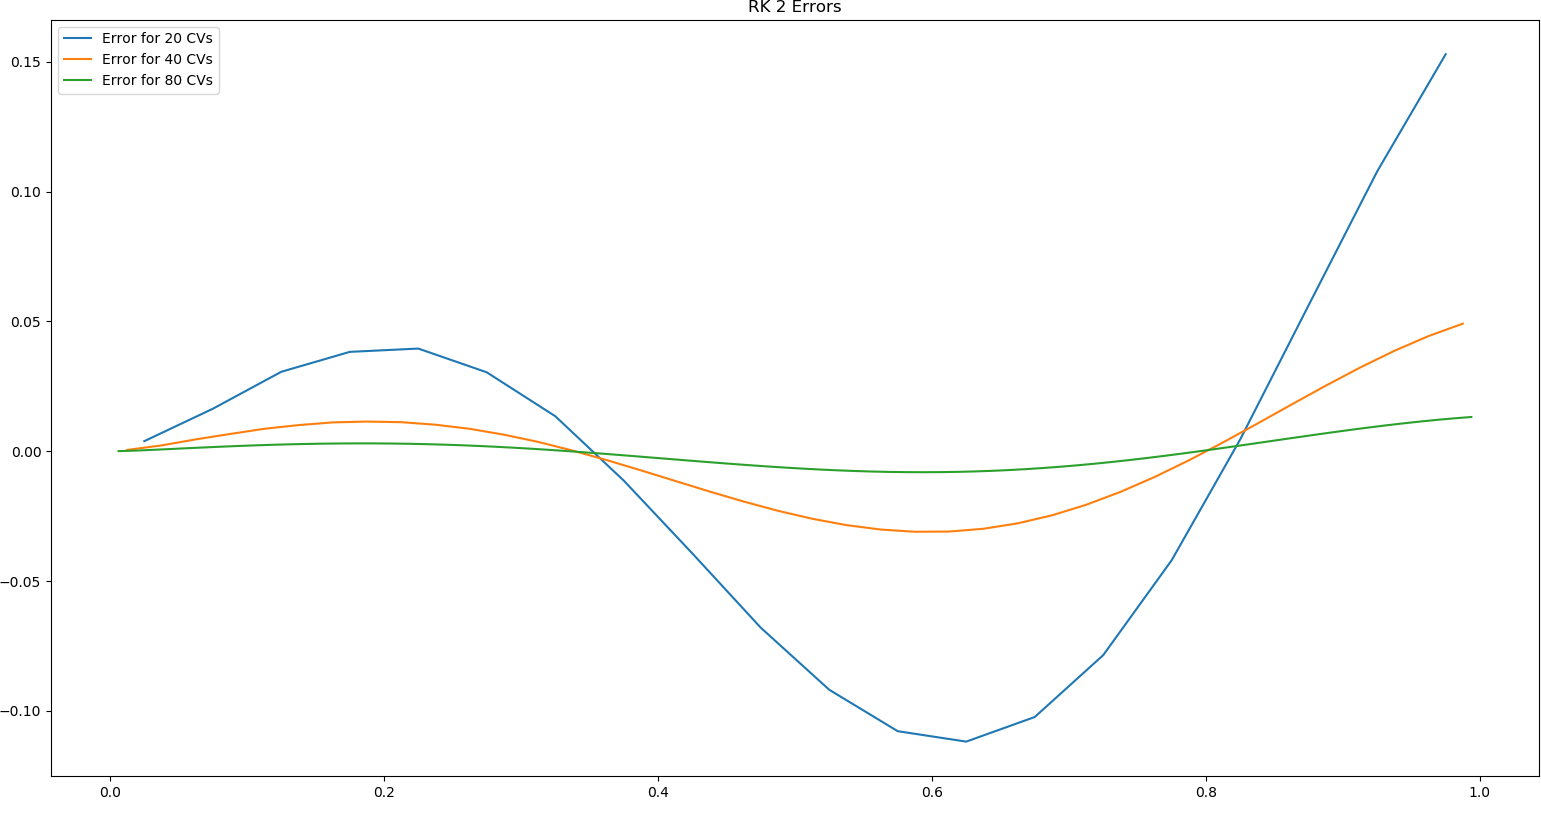
\includegraphics[width=0.7\textwidth]{figs/part1_rk2.png}
  }
  \caption{Errors in the solutions}
  \label{rk_errors}
\end{figure}

I also attempted to determine at what mesh sizes the $L_2$ error reaches certain milestones.
Specifically, I found that the $L_2$ error reaches 1e-3 between 1108 and 1110 control volumes,
and it reaches 1e-4 between 5160 and 5162 control volumes.
For second order convergence, a factor of 10 improvement in error is expected by increasing
the mesh size by a factor of $\sim 3.2$.
The solver doesn't quite reach that level of accuracy,
but is within a factor of 5 which is substantially better than $1^{st}$ order convergence.
The unit tests however show that the extrapolated order of convergence of the average value
is essentially 2, as expected.
\end{section}

\begin{section}{Stability}
Once convinced that the solver was correct, we then considered its stability.
The second order upwinding space discretization has eigenvalues
$\lambda_k = \frac{u}{2 \Delta x} (-3 + 4 e^{-I \phi_k} - e^{-2 I \phi_k})$.
For RK2 to be stable, we need $\lambda_k \Delta t$ to be between $-2$ and $0$ along the real axis
(in general, this is not enough to guarantee stability,
but for this scheme, this is our limiting frequency).
Along the real axis, the space discretization has eigenvalues $0$ and $-4 \frac{u}{\Delta x}$.
Then $-4 \frac{u}{\Delta x}\Delta t = -2$ occurs when we have a CFL number of $0.5$
The same analysis can be performed with the 1st order upwinding scheme to get the same result.

To verify the solver is stable up to this CFL number,
an initial condition was set up with a discontinuity.
This ensures that all frequency modes will be non-negligible so that any modes which the solver
is unstable at will be amplified.
Then, the solver was run with various CFL numbers and $500$ control volumes,
and the solution after 8 units of time was plotted in Figure \ref{stability}.

\begin{figure}[ht]
  \centering{
    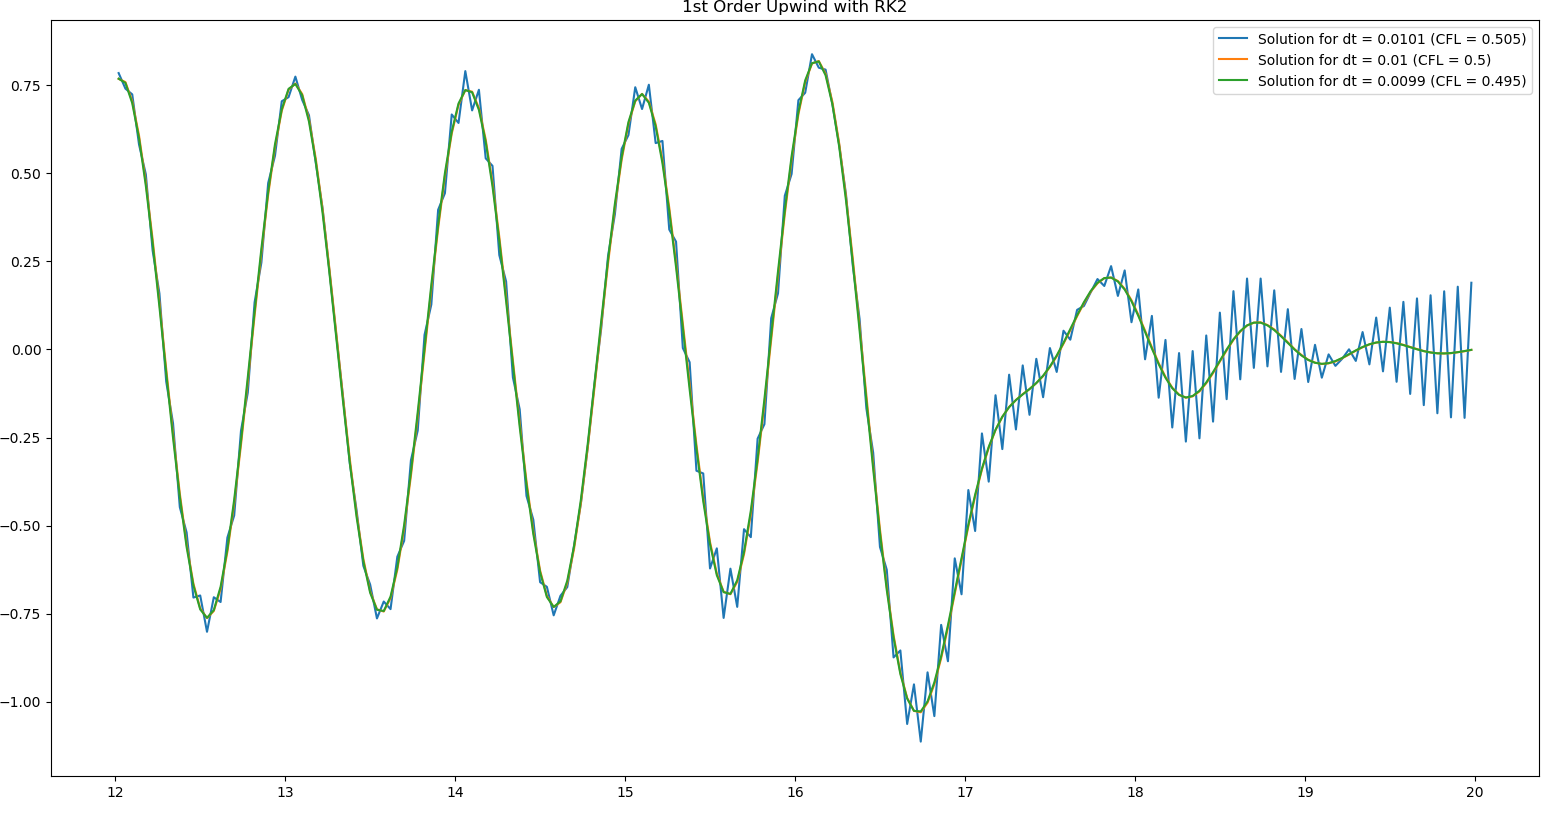
\includegraphics[width=0.7\textwidth]{figs/stability_rk2_1.png}
    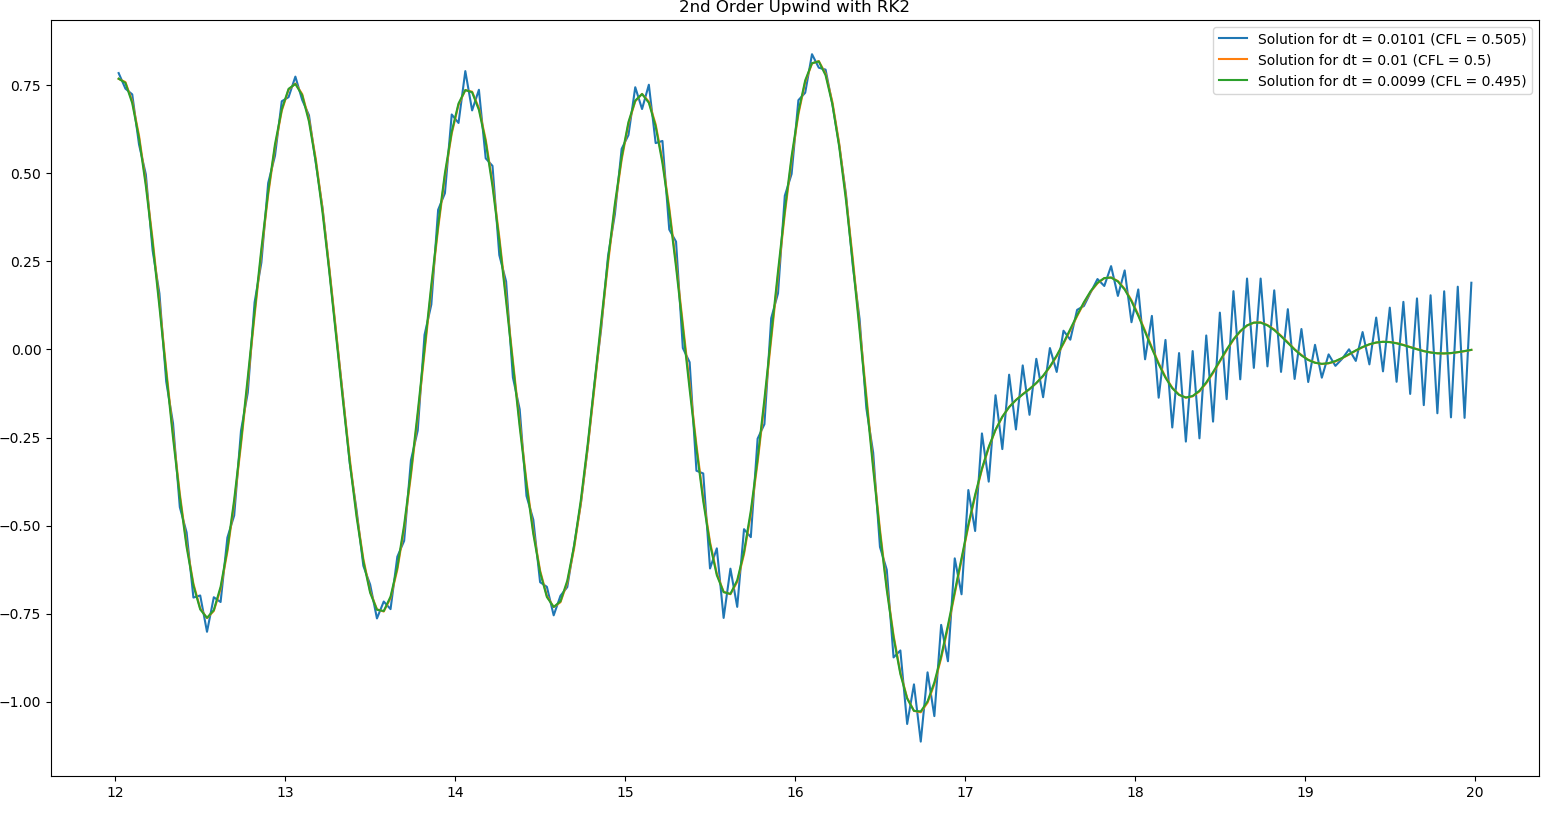
\includegraphics[width=0.7\textwidth]{figs/stability_rk2_2.png}
  }
  \caption{Solution stability for various CFL numbers}
  \label{stability}
\end{figure}

For this level of discretization and the CFL numbers plotted,
an unexpected oscillation has appeared in the solution in the
sinusoidal part of the solution with the $0.505$ CFL number.
This is an indication that it's unstable, as the error in the solution
likely contains some of the frequency modes which will be amplified and grow without bound.
Had the solution been allowed to continue on,
this would have continued growing until everything else was swamped out.
On the other hand, the solution at the theoretical limit of stability shows no signs of instability,
and is nearly a perfect match of the solution just beneath the theoretical limit.

\end{section}

\begin{section}{Scheme Combinations}
Finally, we consider different combinations of the first and second order
time and space discretization schemes.
For RK1 to be stable,
we need $\lambda_k \Delta t$ to be within the unit circle centered at $-1 + I 0$.
The eigenvalues for the first order upwinding scheme are given by
$\lambda_k = \frac{u}{\Delta x} (-1 + e^{-I \phi_k})$.
This is a circle of radius $\frac{u}{\Delta x}$ centered at $-1 + I 0$.
Then for it to be stable with RK1, $\frac{u}{\Delta x} \Delta t < 1$.
For it to be stable with RK2,
$\lambda_k \Delta t$ must be within the region in Figure \ref{rk2_region}.
This is clearly true for the unit circle centered at $-1 + I 0$,
so we conclude that this should be stable for a CFL number of $1$.

\begin{figure}[ht!]
  \centering{
    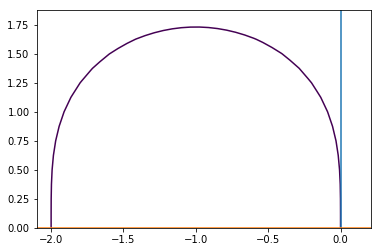
\includegraphics[width=0.3\textwidth]{figs/region_stability_rk2.png}
  }
  \caption{Region of stability for RK2}
  \label{rk2_region}
\end{figure}

Figure \ref{time_errs} shows the plot of the $L_1$ and $L_{\inf}$ errors
with respect to simulated time for a mesh with 80 control volumes and
CFL numbers which are at $80\%$ of the stable limit.

\begin{figure}[ht]
  \centering{
    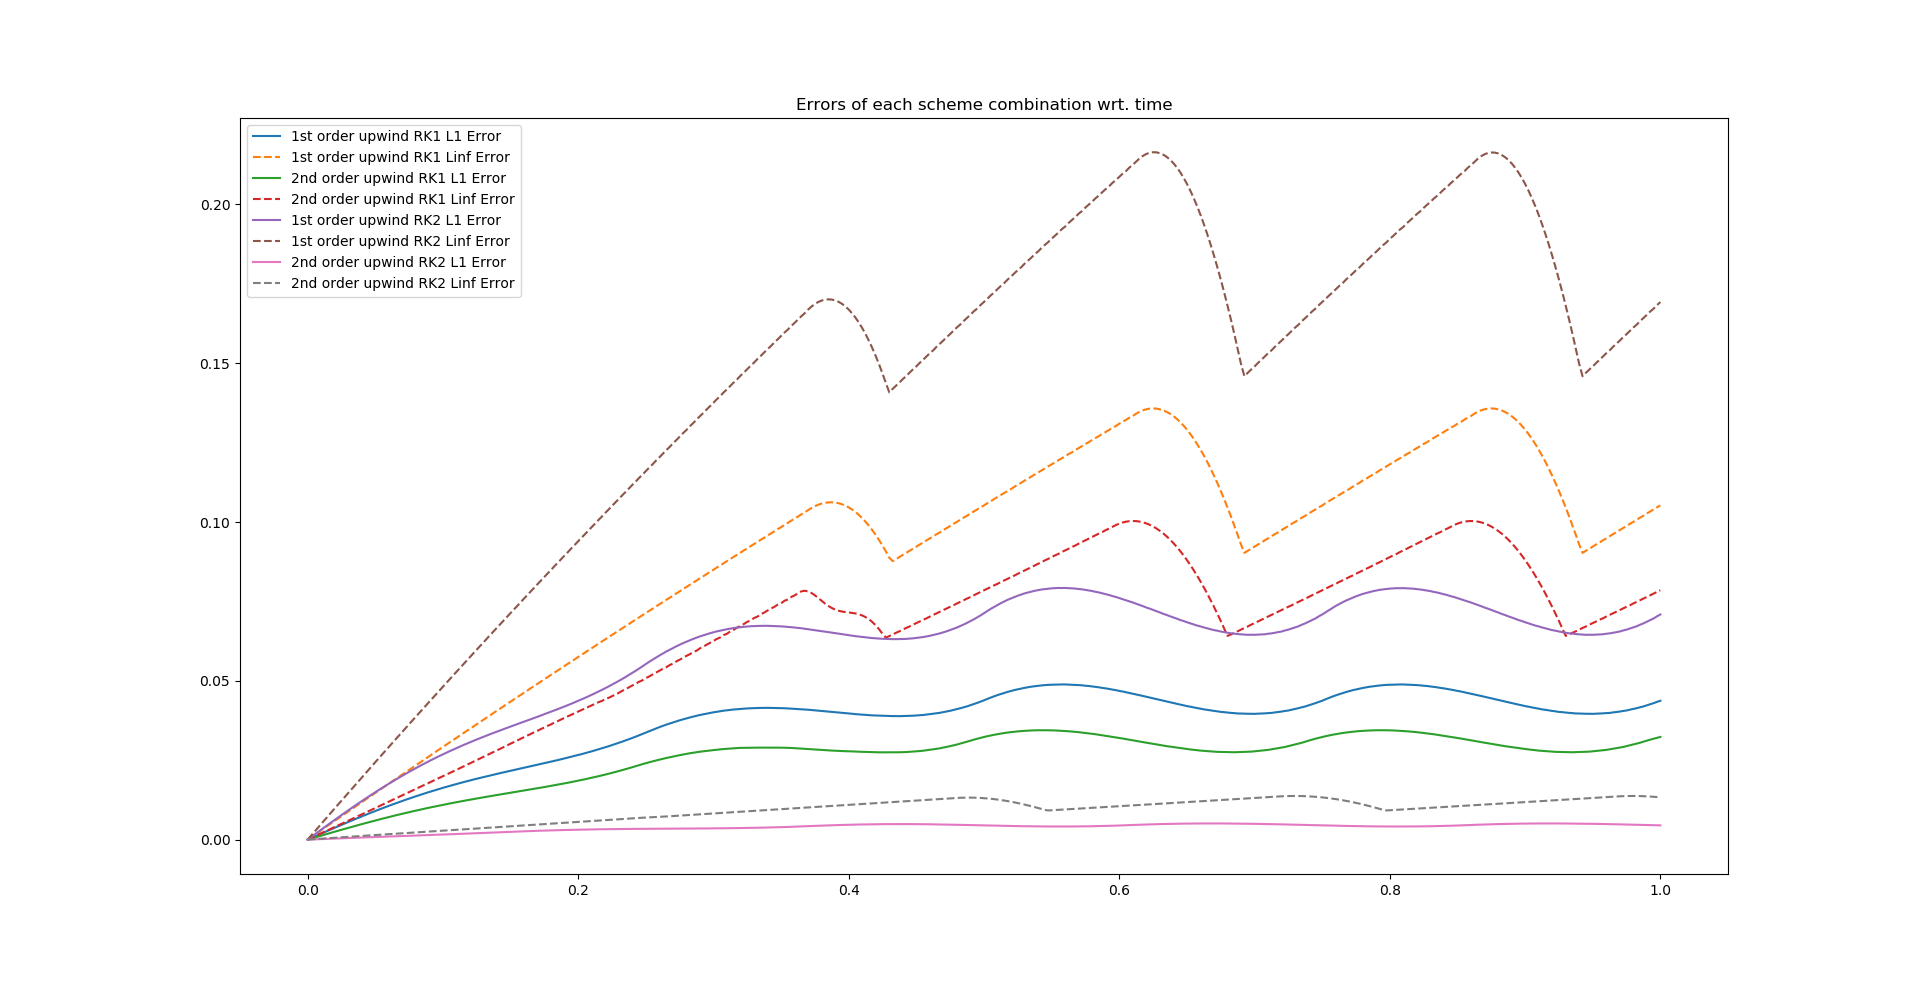
\includegraphics[width=0.95\textwidth]{figs/part3_errs_time.png}
    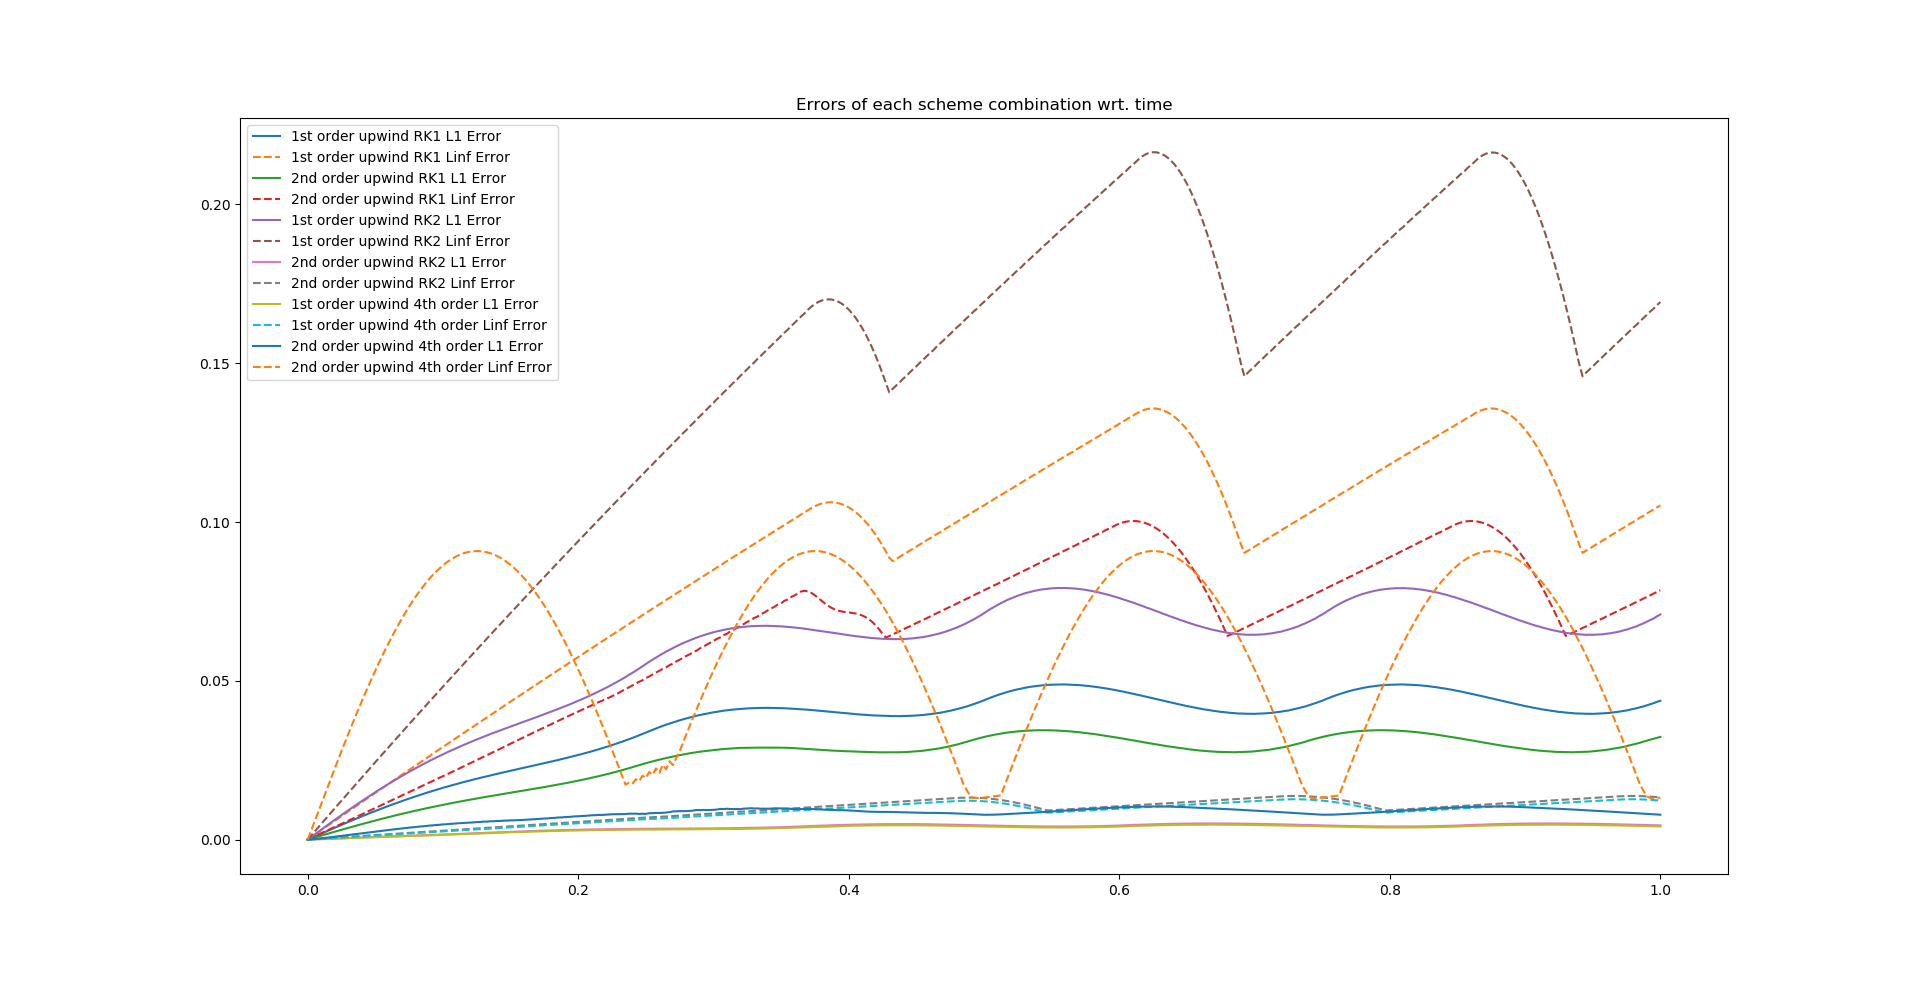
\includegraphics[width=0.95\textwidth]{figs/part3_errs_time_rk4.png}
  }
  \caption{Error with time; first without rk4, second with rk4}
  \label{time_errs}
\end{figure}

Figure \ref{space_errs} shows the plot of the $L_1$ and $L_{\inf}$ errors
with respect to increasing mesh size at time $t = 1.0$.
These were also run with CFL numbers which are at $80\%$ of the stable limit of the scheme.
The slope of the lines shows the rate of convergence of the schemes; more negative is better.
The mesh sizes used were of the form $10 \times 2^n$, with a maximum of 320.
Clearly, the best scheme is RK2 with second order upwinding;
surprisingly RK4 with second order upwinding doesn't have as steep a slope,
and only seems to get first order convergence.

\begin{figure}[ht]
  \centering{
    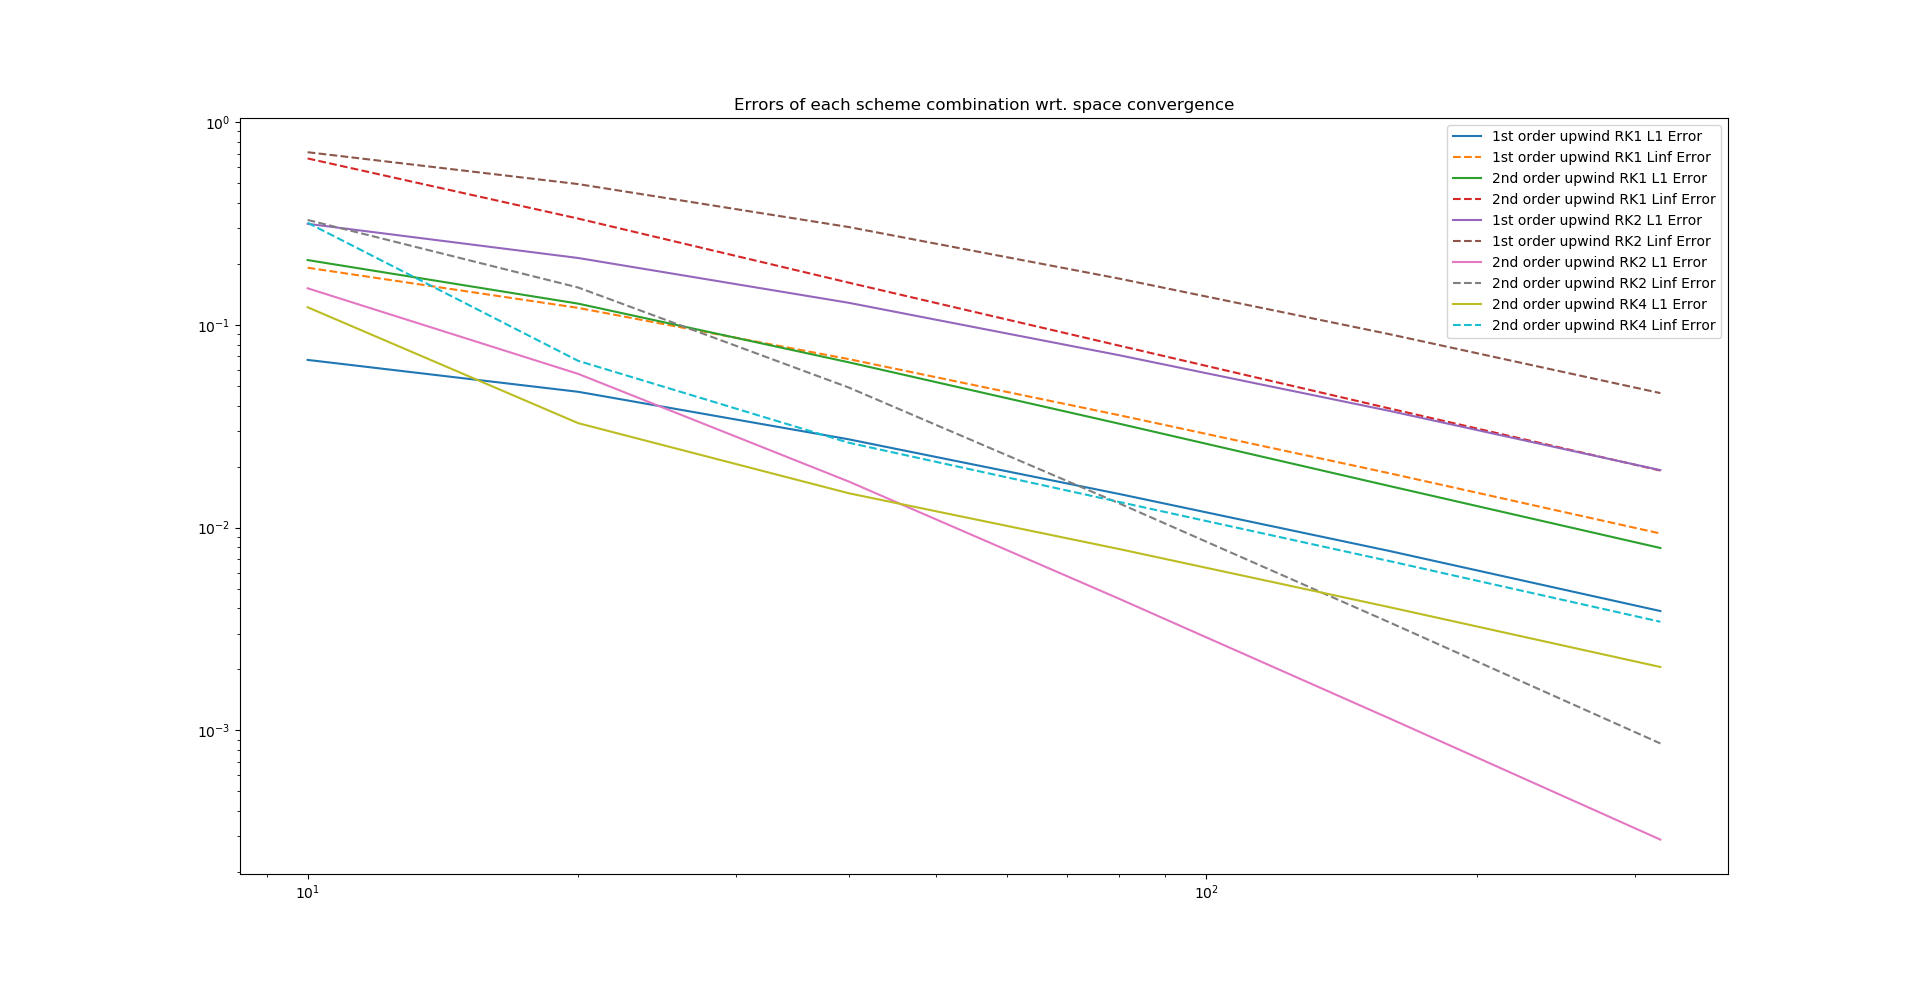
\includegraphics[width=0.95\textwidth]{figs/part3_errs_space_loglog_rk4.png}
  }
  \caption{Error with mesh size}
  \label{space_errs}
\end{figure}
\end{section}

\end{document}
